\section*{Primera Vuelta}
\subsection*{Barrido del Espectro FM}
En Argentina, la banda de frecuencias para el servicio de FM se encuentra entre los $88MHz$ y los $108MHz$. Utilizando el analizador de espectro, se realizó un barrido de frecuencias en la banda de FM, y se eligió la frecuencia de \textbf{$103.7MHz$}. 
Se muestra en la siguiente imagen el espectro cuando se posiciona el filtro pasa-banda centrado en la frecuencia de la portadora y con un ancho de banda de $264kHz$.
\begin{figure}[H]
    \centering
    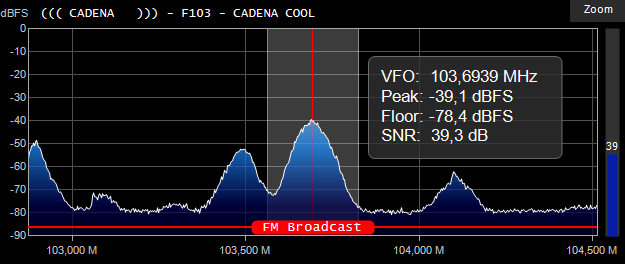
\includegraphics[width=0.9\columnwidth]{images/1.1-rds-103.4MHz.png}
    \caption{Espectro de la frecuencia $103.7MHz$}
    \label{fig:imagen1}
\end{figure}
En esta frecuencia, se pudo observar gracias al plugin \textbf{\textit{FM MPX Spectrum}} que el espectro no es esencialmente el audio en la banda de $0 \sim 15kHz$. Lo que se tiene es la señal \textbf{MPX} que utiliza los dos canales de audio (L y R) para formar el espectro de la imagen \hyperref[fig:imagen2]{Imagen 2}:
\begin{itemize}
	\item El espectro de la suma de los canales.
	\item La frecuencia piloto de $19kHz$.
	\item El espectro de la resta de los canales que posteriormente es modulado en AM para centrarlo en $38kHz$
	\item Y finalmente, el espectro del mensaje RDS que es un mensaje digital que se modula y se agrega al espectro.
\end{itemize}
Dado que el espectro llega mas allá de los $15kHz$, el ancho de banda de Carson ahora será de $264kHz$ ya que si la banda base es de $W=57kHz$, y la máxima desviación de frecuencia se define en $75kHz$, entonces:
$$
BW_{c} = 2\left( \dfrac{75kHz}{57kHz}+ 1 \right) \cdot 57kHz = 264kHz
$$
Por este motivo, se utilizó anteriormente el filtro pasa-banda con un ancho de banda igual a $BW_{c}$.
\begin{figure}[H]
    \centering
    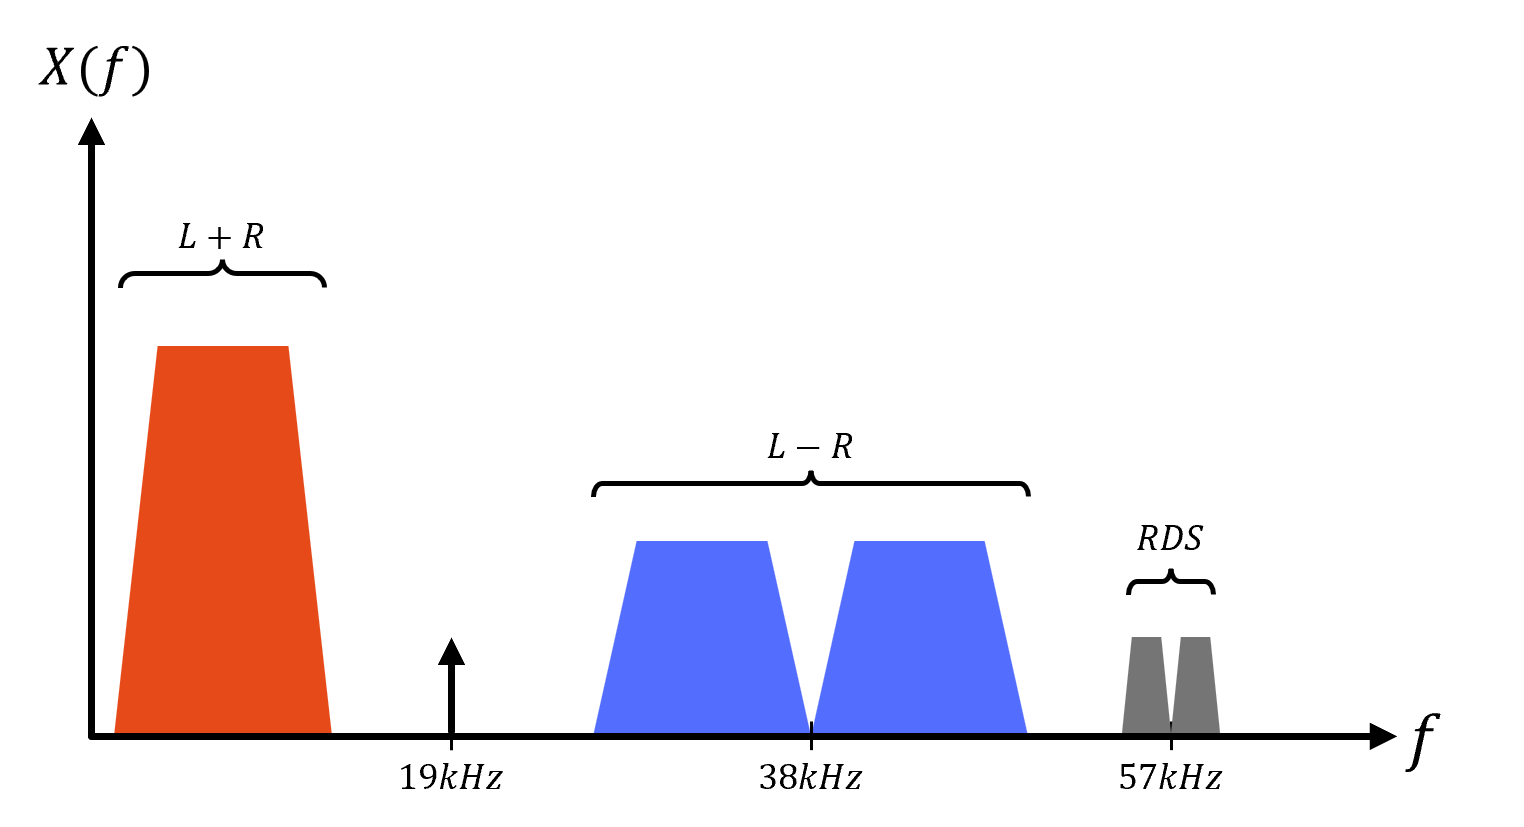
\includegraphics[width=0.8\columnwidth]{images/1.2-espectro-mpx.png}
    \caption{Espectro de una señal MPX}
    \label{fig:imagen2}
\end{figure}

El hecho de ir reduciendo la banda de paso del filtro provoca que se reciba menos potencia de la señal, lo que se traduce en una menor relación señal a ruido, de esta forma se puede observar que la señal de audio se va perdiendo a medida que se reduce el ancho de banda del filtro.

\begin{figure}[H]
    \centering
    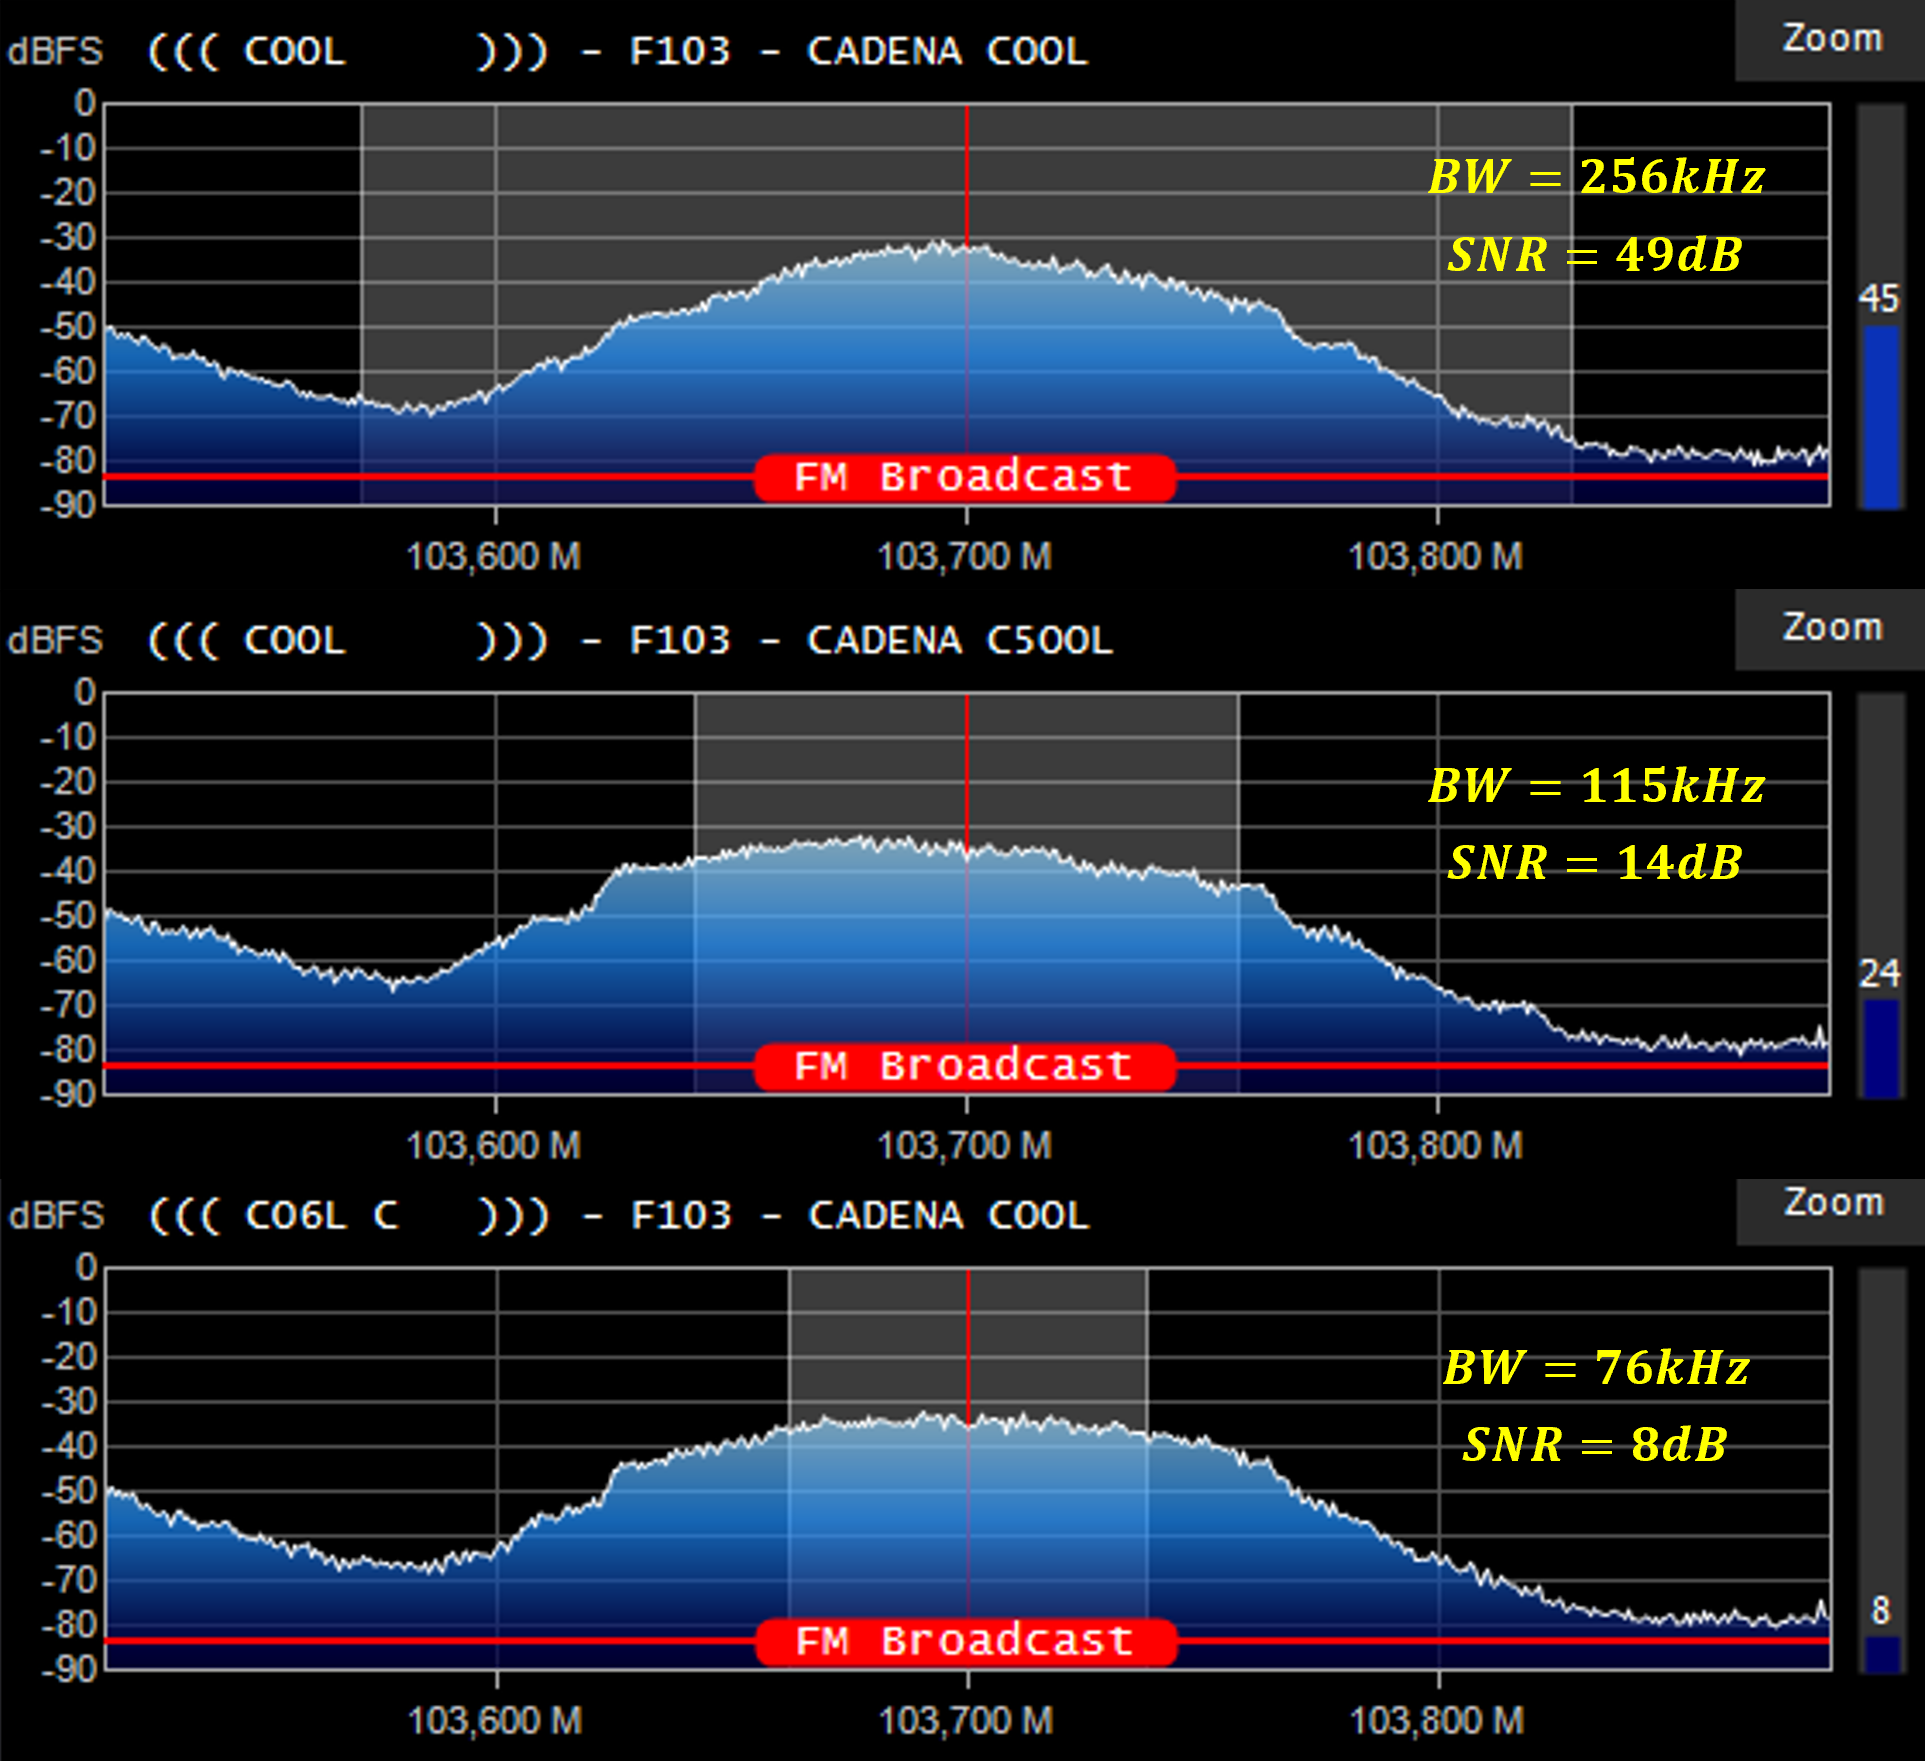
\includegraphics[width=0.9\columnwidth]{images/1.3-mod-bw.png}
    \caption{SNR con distintos anchos de banda}
    \label{fig:imagen3}
\end{figure}

Si la disminución es tal que se pierde parte del espectro de la resta de los canales (L-R en la \hyperref[fig:imagen2]{Imagen 2}), entonces ya no se podrá demodular y escuchar en modo Estéreo.

En el caso de aumentar o disminuir la ganancia del receptor SDR, se puede observar que la señal de audio se distorsiona, y es en parte por aumentar la potencia de ruido, el cual hace que supere en algunos casos la potencia de las estaciones que transmiten.